\documentclass[18pt]{beamer}
\usepackage{templates/beamerthemekit}
\usepackage[export]{adjustbox}
\usepackage{tikz}
\usepackage{bbm}

\usepackage{latexsym,amsmath,amssymb,mathtools,textcomp}
% \usepackage{templates/beamerthemekitwide}

%\titlelogo{mylogo}
% \usepackage{templates/tikzkit}
% \usepackage{templates/tikzuml}
% \titleimage{myimage}


\titlelogo{myimage}


\title[Short title]{Erstellung und Evaluierung stochastischer Regressionsmodelle auf Basis heterogener Messnetzwerke.}
\subtitle{Bachelor Arbeit, Betreuer - Dr. Johannes Riesterer, Dr. Sebastian Lerch}
\author{Stanislav Arnaudov}

\institute{TECO - Das Telecooperation Office}
\usepackage[citestyle=authoryear,bibstyle=numeric,hyperref,backend=biber]{biblatex}
\addbibresource{templates/example.bib}
\bibhang1em
 
\begin{document} 

% \selectlanguage{english}
\selectlanguage{ngerman}


\begin{frame}
 \titlepage
\end{frame}

\begin{frame}
  \frametitle{Motivation}
  
  Given is a heterogeneous network of sensors -- the network contains good \underline{and} bad sensors.\\
  Interesting Questions:
  \begin{itemize}
  \item Can we use the bad sensors in order to predict the values of the good ones?
  \item Can we identify the weak parts of the network?
  \end{itemize}
  Our approach to the problems:
  \begin{itemize}
  \item Use of stochastic regression models.
  \item Formal evaluation of models through the use of proper scoring rules, verification rank histograms and predictive performance checks.
    \item Analyzing the relevancy of each predictor for the final prediction through the use of feature importance technique.
  \end{itemize}
  
\end{frame}

\begin{frame}
  \frametitle{Data}

  \begin{itemize}
  \item Heterogeneous Network of air pollution sensors in Stuttgart.\\
    \begin{itemize}
    \item LU-BW (\textit{Landesanstalt für Umwelt, Messungen und Naturschutz Baden-Württemberg}) - \textbf{3 Sensors} of high Quality.
    \item \textit{luftdaten.info} -- Public data from cheap DIY sensors.
    \end{itemize}
    \item Considered period: the year of 2018.
  \end{itemize}

\end{frame}

\begin{frame}
  \frametitle{Stochastic Regression Models}
  \begin{itemize}
  \item Regression: Feature vector $\mapsto$ a real value
  \item Stochastic Regression: Feature vector $\mapsto$ a real value
  \end{itemize}
  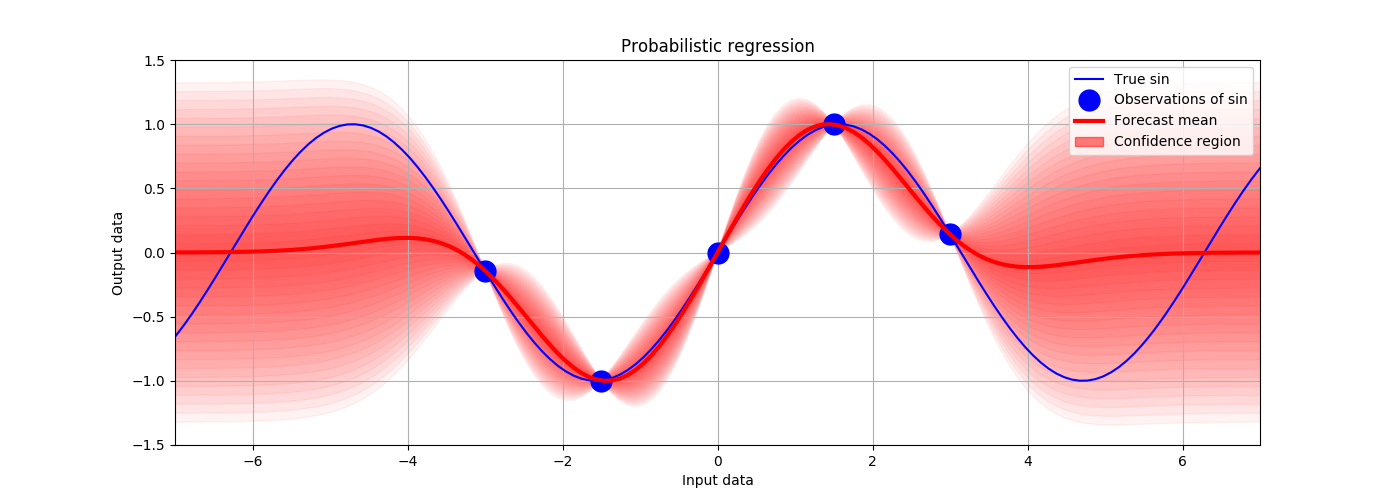
\includegraphics[scale=0.35]{images/probabilistic_regression}
  
\end{frame}

\begin{frame}
  \frametitle{General View}
  \begin{center}
  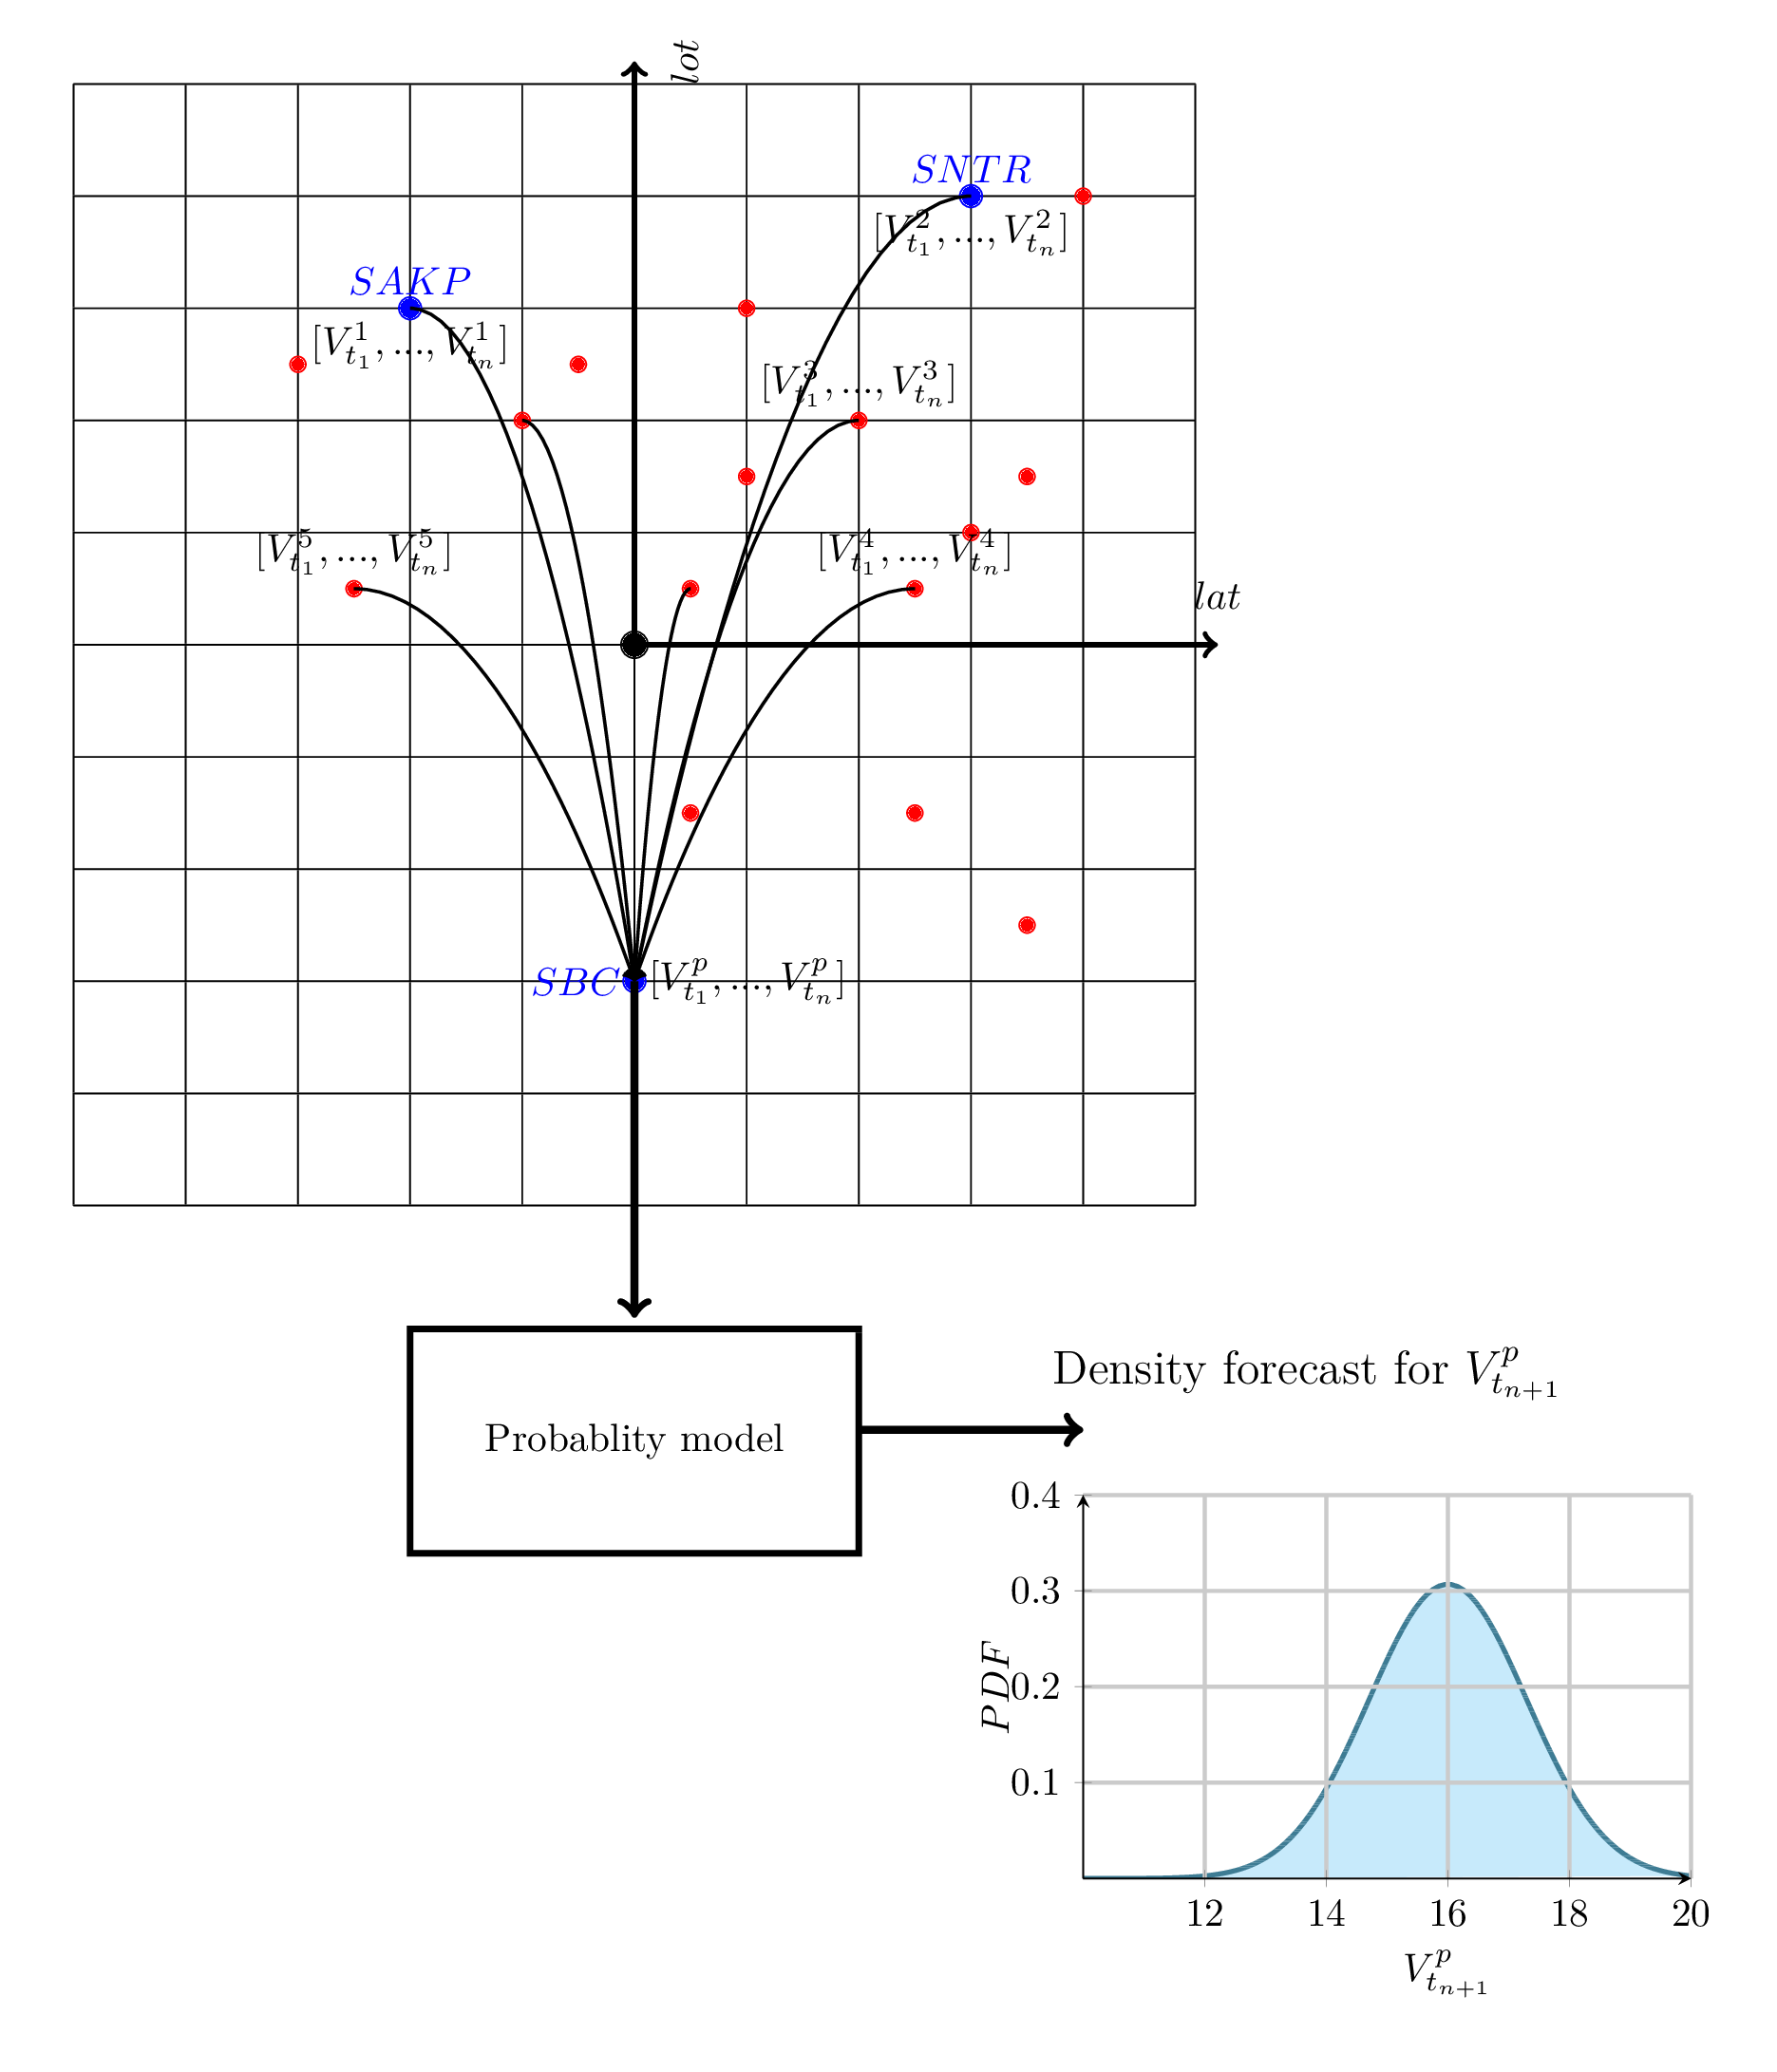
\includegraphics[scale=0.10]{images/general_system}
  \end{center}
\end{frame}


\begin{frame}
  \frametitle{Concrete Models}
  
  \begin{itemize}
  \item Bayesian Neural Networks
  \end{itemize}
  \begin{center}
    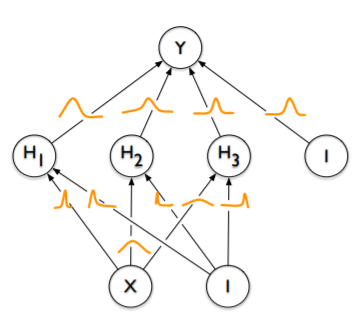
\includegraphics[scale=0.5]{images/bnn}
  \end{center}
  
\end{frame}

\begin{frame}
  \frametitle{Concrete Models}
  
   \begin{itemize}
   \item Mixture Density Networks
   \end{itemize}

   \begin{center}
     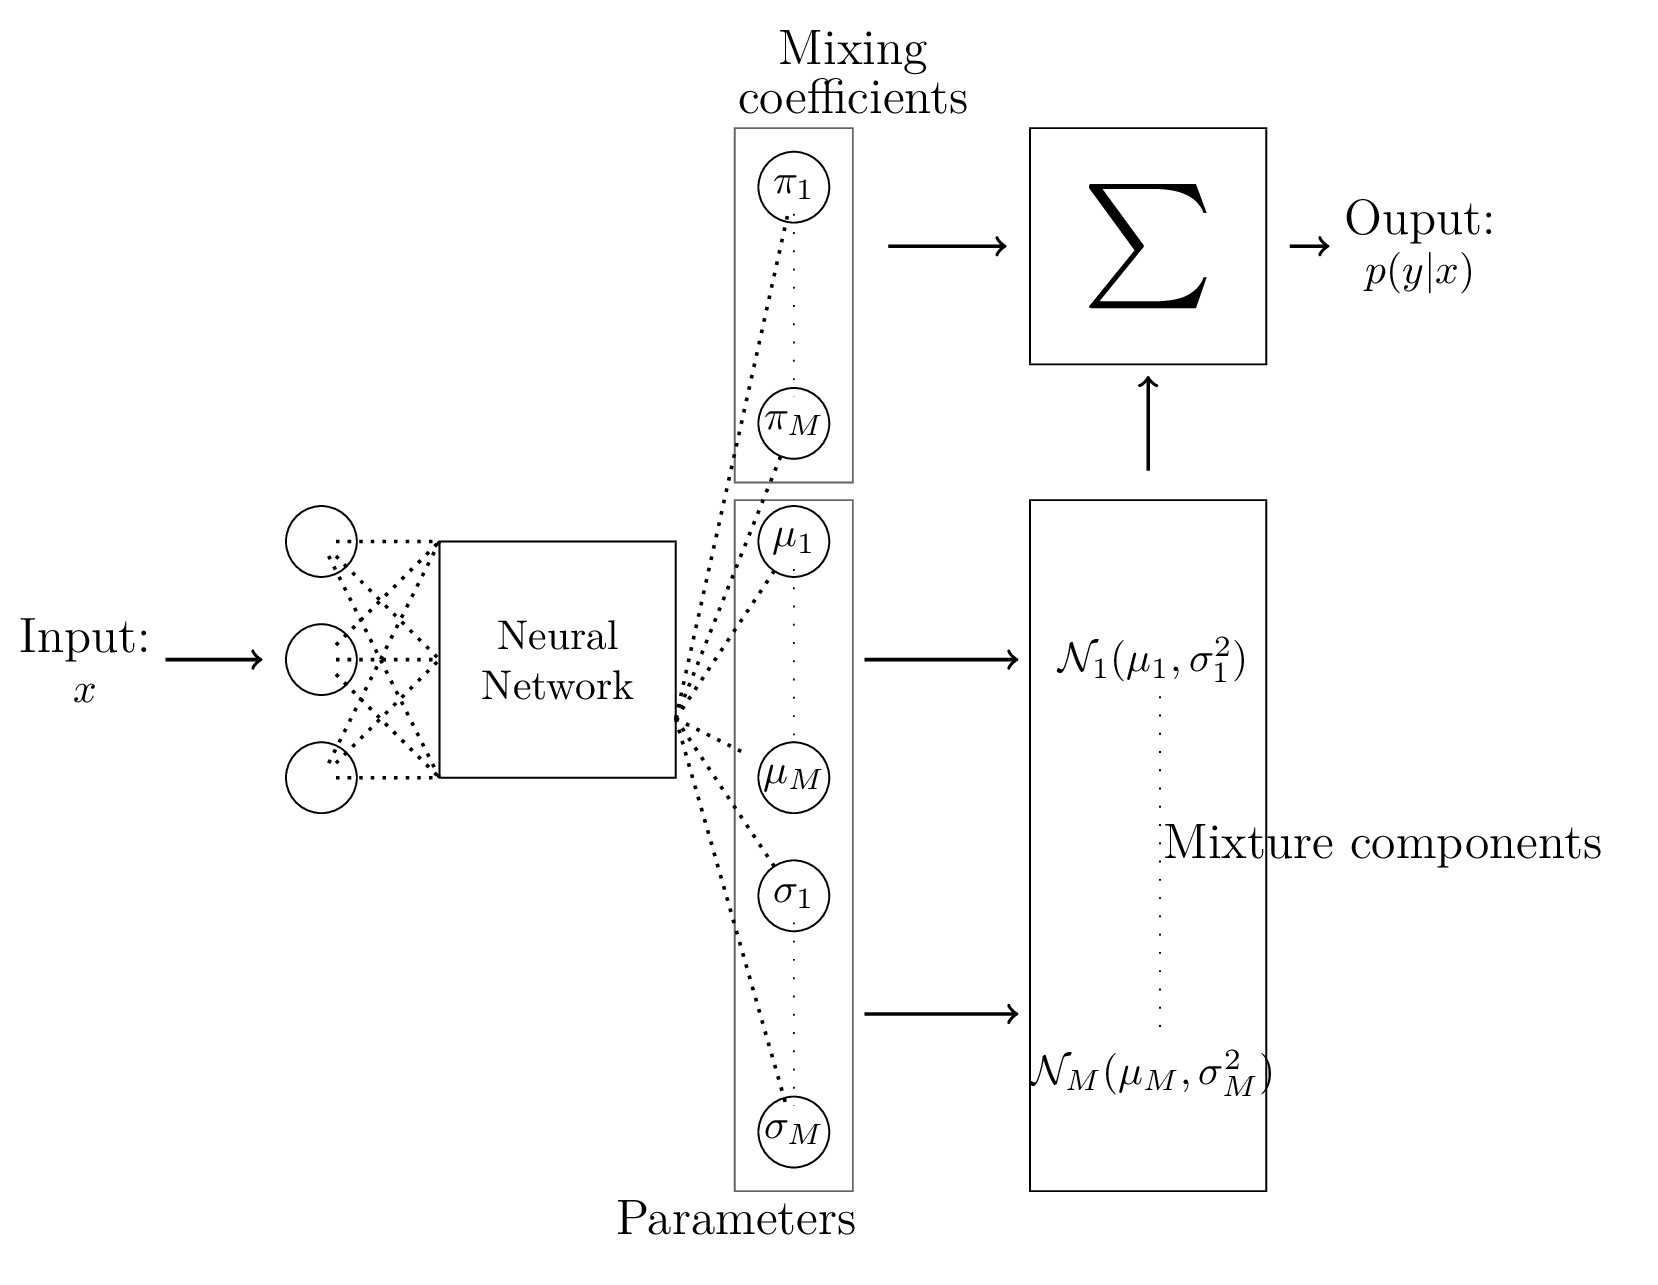
\includegraphics[scale=0.15]{images/mdn}
   \end{center}
  
 \end{frame}

\begin{frame}
  \frametitle{Concrete Models}
  Empirical model
   \begin{itemize}
   \item Passed observations are treated as values of a random variable and from that a distribution for the predicted observation is implied.
   \item We used this model as a baseline.
   \item We hopped to achieve better than the empirical model results with the other two models.
   \end{itemize}

 \end{frame}

\begin{frame}
  \frametitle{Evaluation of probability distributions}
  \begin{itemize}
  \item We do not compare point estimate with a realized real value but rather a probability distribution with real value.
  \end{itemize}
  \begin{center}
    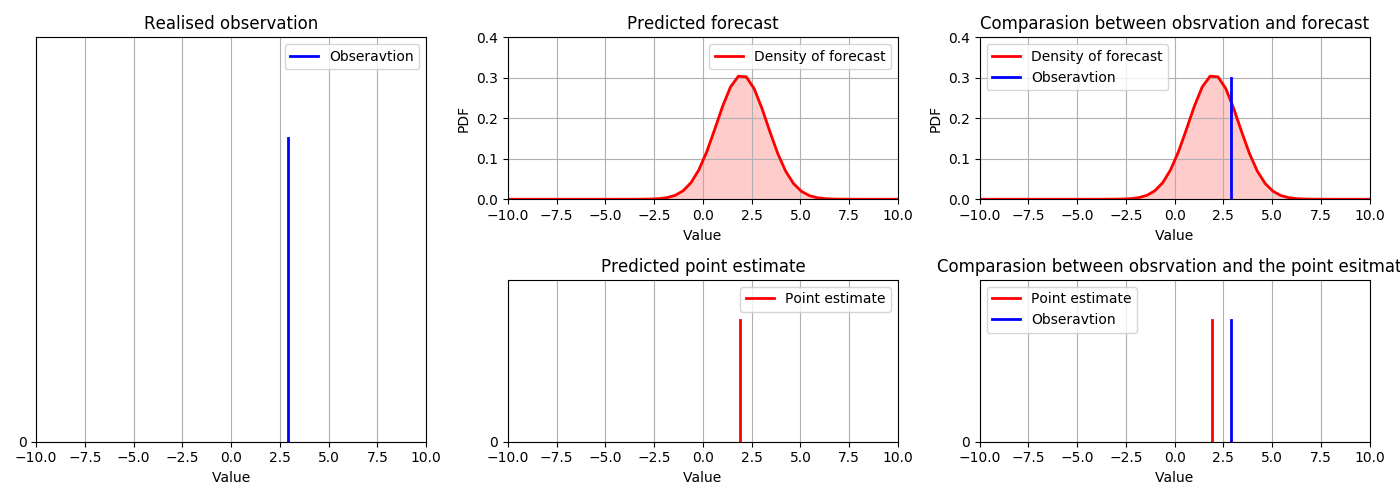
\includegraphics[scale=0.32]{images/distribution_point}
  \end{center}
\end{frame}

\begin{frame}
  \frametitle{Continuous Rank Probability Score}
  \begin{itemize}
  \item CRPS a distribution with the observation, where both are represented as cumulative distribution functions.
    $$  CRPS(F,y)  = \int_{-\infty}^{\infty}(F(x) - \mathbbm{1}\{y \leq x \})^2dx $$
  \end{itemize}
  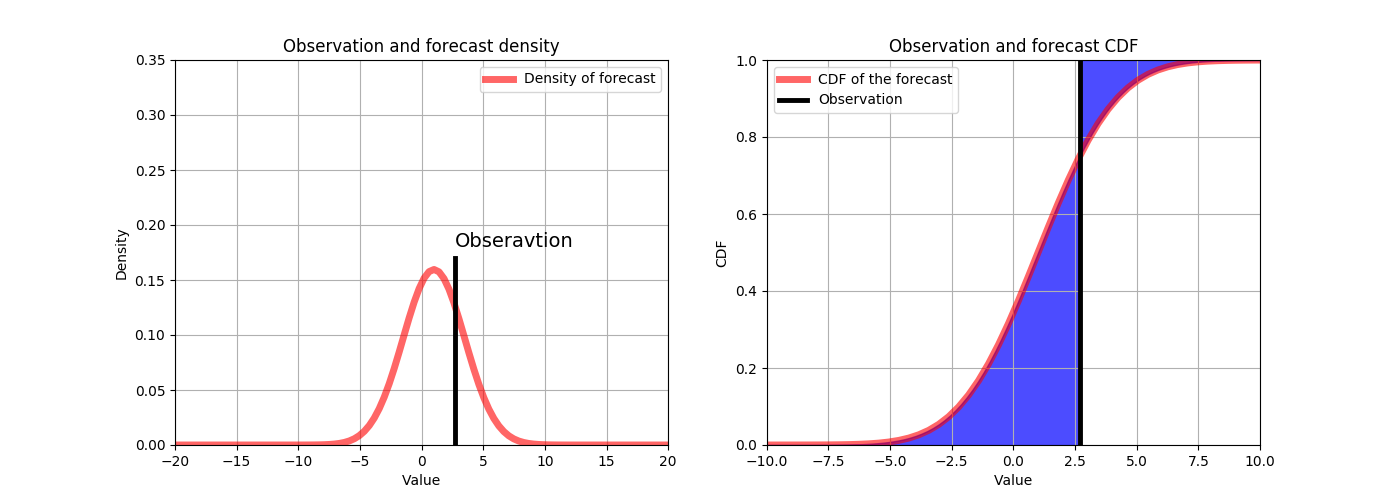
\includegraphics[scale=0.35]{images/crps}
\end{frame}

\begin{frame}
  \frametitle{Rank Verification Histograms}
  \begin{center}
    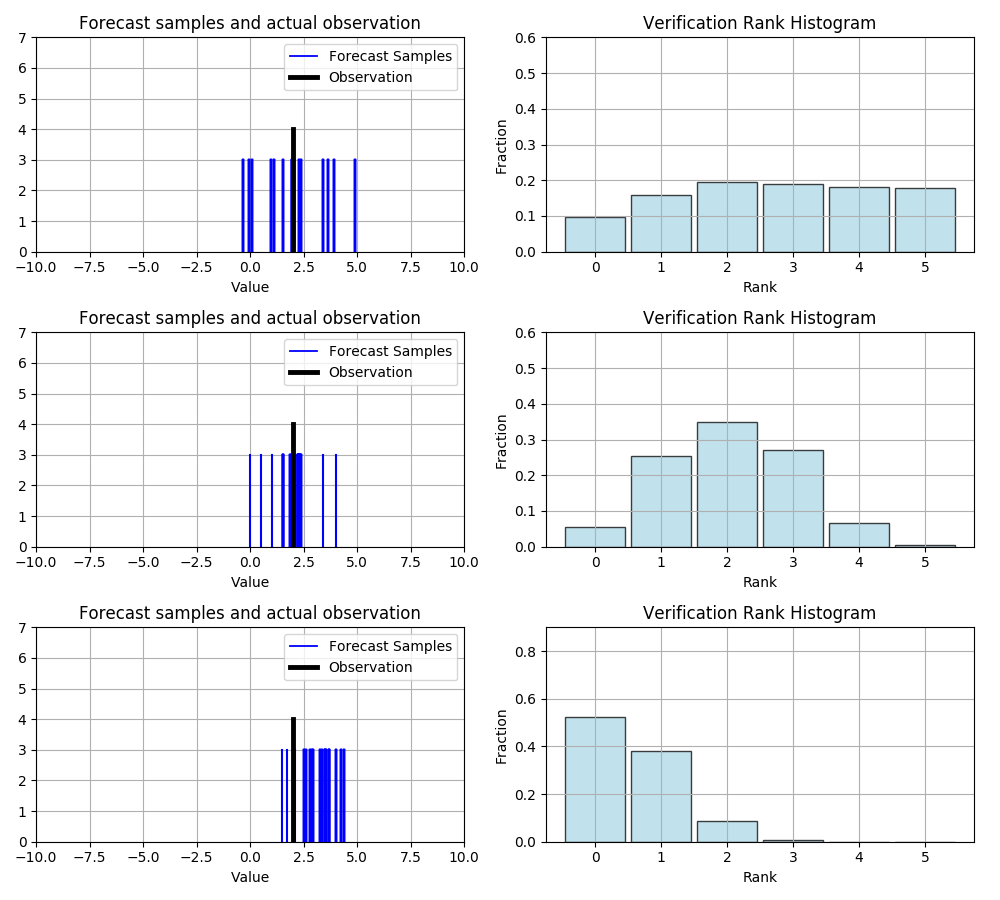
\includegraphics[scale=0.32]{images/verification_histogram}
  \end{center}
\end{frame}


\end{document}

%%% Local Variables:
%%% mode: latex
%%% TeX-master: t
%%% End:
